\documentclass[english]{article} 
\usepackage{geometry}
\geometry{hmargin=2.1cm,vmargin=3.5cm}
\usepackage{multicol}
\usepackage{lipsum}
\usepackage{graphicx}
\usepackage[hidelinks]{hyperref}
\usepackage[utf8]{inputenc}
\usepackage{babel}
\usepackage[T1]{fontenc}
\usepackage{textcomp}
\usepackage{lmodern, newunicodechar}
\usepackage{textgreek}
\usepackage{url}
\usepackage{enumitem}
\usepackage{minted}
\usepackage{amsmath}
\usepackage{mathtools}
\usepackage{mathrsfs}
\usepackage{sistyle}
\usepackage{csvsimple}
\usepackage{caption}



\begin{document}

\begin{titlepage}

    \begin{center}
        
\includegraphics[scale=0.05]{rsc/logos/LOGO-UNIV-FC_COULEUR.png}
        \hspace{1cm}
        
\includegraphics[scale=0.025]{rsc/logos/utinam.png}
        \hspace{1cm}
        
\includegraphics[scale=0.04]{rsc/logos/CNRS.png}
        \hspace{1cm}
        
\includegraphics[scale=0.04]{rsc/logos/femto.png}
        \hspace{1cm}
    \end{center}

    \vbox{ }

    \vbox{ }

    \begin{center}
        % Øverste del av siden
                
        \textsc{\Large Free Project Techhnical Report - M2 CompuPhys}\\[1cm]

        % \vbox{ }
        % Tittel
        \noindent\makebox[\linewidth]{\rule{.7\paperwidth}{.6pt}}\\[0.7cm]
        { \Huge \bfseries - Technical Report - \\ Implementation of Direct Feedback Alignment Using PyTorch}\\[0.25cm]
        \noindent\makebox[\linewidth]{\rule{.7\paperwidth}{.6pt}}\\[0.7cm]
        \LARGE{Léo BECHET}\\
        \small{University of Franche-Comté}\\[1.2cm]
        
        \vfill
        % Forfatter
        \large
        % \emph{Skrevet av:}\\[1mm]
        \Large{Under the supervision of Pr.Daniel BRUNNER,\\
        and Dr.Anas SKALLI from the FEMTO-ST Institute}

        % Nederste del av siden
    \end{center}
\end{titlepage}

\newpage
\tableofcontents
\newpage

% Mise en page pour l'abstract
\section*{\centering \textbf{Abstract}}

\begin{center}
  \hrulefill\\[0.2cm]
  \begin{minipage}{0.9\textwidth}
      \centering
      This project aims to evaluate the effectiveness of Direct Feedback Alignment (DFA) as an alternative to backpropagation in training neural networks, particularly focusing on its applicability to batched data. Averaging on batches aims to lower the sampling cost. We introduce various averaging techniques for batch processing to better align with experimentally plausible models. The study contrasts DFA with traditional backpropagation by implementing both methods on simple and complex tasks. Specifically, we use the XOR problem as a proof of concept to demonstrate basic functionality and then transition to the MNIST dataset for a more rigorous and complex validation. These tests will provide insights into the performance, stability, and efficiency of DFA compared to backpropagation across different scales of complexity in neural network training.\\
      \textbf{Keywords: Direct Feedback Alignment, Backpropagation, Machine Learning, Neural Network Training.}

  \end{minipage}\\[0.2cm]
  \hrulefill
\end{center}











\section{McCulloch and Pitts Neuron}

The \textbf{McCulloch and Pitts (MCP) neuron}\cite{mcculloch43a} is one of the earliest models in artificial neural networks. It was introduced by Warren S. McCulloch and Walter Pitts in 1943 to formalize the functioning of neurons in biological brains.

\subsection{Mathematical Model}

The MCP neuron operates on a set of input signals, each weighted according to its importance. The neuron's output is determined based on whether the weighted sum of these inputs exceeds a certain threshold.

Given \( n \) input signals \( x_1, x_2, \ldots, x_n \), each with corresponding weights \( w_1, w_2, \ldots, w_n \), and a bias term \( b \), the MCP neuron's output is given by:

\[
y = 
\begin{cases} 
1 & \text{if } \sum_{i=1}^{n} w_i x_i + b > 0 \\
0 & \text{otherwise}
\end{cases}
\]

Here, \( y \) represents the binary output of the neuron (1 for "firing" or "activated," and 0 for "not firing").

\subsection{Training Process}

The training process involves adjusting the weights and bias to minimize errors. This is done using a set of input-output pairs where each pair consists of an input vector \( \mathbf{x} = [x_1, x_2, \ldots, x_n] \) and its corresponding desired output \( t \).

The goal is to find the optimal weights \( \mathbf{w} = [w_1, w_2, \ldots, w_n] \) and bias \( b \) such that the neuron's output matches the desired output for all training examples.

\subsubsection{Learning Rule}

A simple learning rule used in training MCP neurons is the perceptron learning rule. The steps are as follows:

\begin{enumerate}
    \item \textbf{Initialization}: Start with random initial weights $\mathbf{w}_0$ and bias $b_0$.
    
    \item \textbf{Iteration}:
        \begin{itemize}
            \item For each input-output pair $(\mathbf{x}, t)$:
                \begin{enumerate}
                    \item Compute the weighted sum: \( z = \sum_{i=1}^{n} w_i x_i + b \).
                    \item Determine the output of the neuron:
                        \[
                        y = 
                        \begin{cases}
                            1 & \text{if } z > 0 \\
                            0 & \text{otherwise}
                        \end{cases}
                        \]
                    \item If the output does not match the desired output (i.e., $y \neq t$):
                        \begin{enumerate}
                            \item Adjust the weights and bias:
                                \[
                                w_i \leftarrow w_i + \eta (y-t) x_i
                                \]
                                \[
                                b \leftarrow b + \eta (y-t)
                                \]
                            where $\eta$ is a small positive constant known as the learning rate.
                        \end{enumerate}
                \end{enumerate}
        \end{itemize}
    
    \item \textbf{Termination}: Repeat the iteration until all input-output pairs are correctly classified or a maximum number of iterations is reached.
\end{enumerate}
\subsubsection{Convergence}

The perceptron learning rule guarantees that if the training data is linearly separable (i.e., there exists a hyperplane that can separate the two classes), the weights and bias will converge to values that correctly classify all input-output pairs.

\subsection{Example}

Consider a simple example with two inputs \( x_1 \) and \( x_2 \), and desired outputs for training examples as follows:

\begin{enumerate}
\item \textbf{Input}: \(\mathbf{x}_1 = [1, 0]\), Desired Output: \( t_1 = 1 \)
\item \textbf{Input}: \(\mathbf{x}_2 = [0, 1]\), Desired Output: \( t_2 = 0 \)
\end{enumerate}

Starting with random weights and bias, after several iterations of the perceptron learning rule, the neuron's parameters will converge to values that correctly classify these inputs.
\[
\boxed{
\begin{aligned}
&\text{Initial weights: } w_1 = 0.5, w_2 = -0.5, b = 0 \\
&\text{After training, let's assume: } w_1 = 0.6, w_2 = -0.4, b = 0.3
\end{aligned}
}
\]

These values would ensure the neuron correctly outputs \( t_1 = 1 \) for \(\mathbf{x}_1\) and \( t_2 = 0 \) for \(\mathbf{x}_2\).

This completes the presentation of the McCulloch and Pitts neuron, including its mathematical model and training process.




























\section{Multi-Layer Perceptron (MLP)}

\subsection{Introduction}
The Multi-Layer Perceptron (MLP)\cite{rosenblatt1958perceptron} is a fundamental type of artificial neural network. It consists of multiple layers of nodes connected in a feedforward manner, with each node applying a weighted sum and an activation function to its inputs.

\subsection{Neuron Model}
A single neuron in the MLP is an extension of the McCulloch and Pitts neuron and can be mathematically modeled as follows:

\begin{equation}
    z = \sum_{j=1}^{n} w_j x_j + b
\end{equation}

where:
\begin{enumerate}[label=]
\item \( z \) is the pre-activation (or net input).
\item \( w_j \) are the weights associated with the inputs.
\item \( x_j \) are the inputs to the neuron.
\item \( b \) is the bias term.
\end{enumerate}
The output of the neuron, often denoted as \( a \), is then passed through an activation function \( f \):

\begin{equation}
    a = f(z)
\end{equation}

Common activation functions include:
\begin{enumerate}[label=]
    \item \textbf{Sigmoid}: \( f(z) = \frac{1}{1 + e^{-z}} \)
    \item \textbf{Tanh}: \( f(z) = \tanh(z) \)
    \item \textbf{ReLU (Rectified Linear Unit)}: \( f(z) = \max(0, z) \)
\end{enumerate}

\subsection{Multi-Layer Perceptron Architecture}
An MLP consists of multiple layers:
\begin{enumerate}
    \item \textbf{Input Layer}: Receives the raw input data.
    \item \textbf{Hidden Layers}: Intermediate layers that transform the input data using a series of neurons with activation functions.
    \item \textbf{Output Layer}: Produces the final output, often corresponding to the class labels or continuous values.
\end{enumerate}

The architecture can be represented as follows:

\begin{equation}
    \text{Input} \xrightarrow{\text{Weights}} \text{Hidden Layers} \xrightarrow{\text{Activation Functions}} \text{Output Layer}
\end{equation}

\subsection{Training the MLP}
Training an MLP involves adjusting the weights and biases to minimize a loss function. This is typically done using an optimization algorithm like gradient descent.

The goal is to find the set of parameters \( \theta = [w, b] \) that minimizes the loss function:

\begin{equation}
    L(\theta; x^{(i)}, y^{(i)}) = \text{Loss Function}(\mathbf{x}^{(i)}, \mathbf{y}^{(i)})
\end{equation}

where:
\begin{itemize}
    \item \( \mathbf{x}^{(i)} \) is the input vector for example \( i \).
    \item \( \mathbf{y}^{(i)} \) is the target output vector for example \( i \).
\end{itemize}

Common loss functions include:
\begin{enumerate}[label=]
    \item \textbf{Mean Squared Error (MSE)}: 
        \[
        L(\theta; x^{(i)}, y^{(i)}) = \frac{1}{2} \| a_L - t \|^2
        \]
    where \( a_L \) is the predicted output and \( t \) is the true target.
    
    This loss function is suitable for regression problems.

    \item \textbf{Binary Cross-Entropy (BCE)}:
        \[
        L(\theta; x^{(i)}, y^{(i)}) = -[y^{(i)} \log(a_L) + (1 - y^{(i)}) \log(1 - a_L)]
        \]
    
    This loss function is suitable for binary classification problems.

    \item \textbf{Root Mean Squared Error (RMSE)}:
        \[
        L(\theta; x^{(i)}, y^{(i)}) = \sqrt{\frac{1}{n} \sum_{i=1}^n (a_L - t)^2}
        \]
    
    This loss function is also a variant of the MSE and is used in regression tasks.
\end{enumerate}

The loss function measures the discrepancy between the network's predictions and the actual targets. It must be wisely chosen to fit the problem the MLP has been tasked to solve.

The training process can be summarized as follows:

\begin{enumerate}
    \item \textbf{Forward Propagation}: Compute the outputs through each layer using the current weights and biases.
    \item \textbf{Compute Loss}: Calculate the loss function for a given set of inputs and targets.
    \item \textbf{Backward Propagation}: Use backpropagation to compute the gradient of the loss with respect to each weight and bias in the network.
    \item \textbf{Update Weights}: Adjust the weights using an optimization algorithm such as stochastic gradient descent (SGD):

\begin{equation}
    w \leftarrow w - \eta \frac{\partial L}{\partial w}
\end{equation}

where \( \eta \) is the learning rate.

    \item \textbf{Repeat Steps 1-4}: Iterate over the training data and update the weights until convergence or a stopping criterion is met.
\end{enumerate}

\subsection{Example Training Process}
Here's an example of the training process for a simple MLP with one hidden layer:

\begin{enumerate}
    \item Initialize random weights \( w \) and biases \( b \).
    \item For each input \( x^{(i)} \):
        \begin{enumerate}
            \item Compute the pre-activation: \( z = \sum_{j=1}^{n} w_j x_j + b \)
            \item Apply the activation function to get the output: \( a = f(z) \)
            \item Calculate the loss and its gradients.
        \end{enumerate}
    \item Update the weights using gradient descent:
\begin{equation}
    w \leftarrow w - \eta \frac{\partial L}{\partial w}
\end{equation}

    \item Repeat steps 2-3 until convergence or a stopping criterion is met.
\end{enumerate}






















\section{Direct Feedback Alignment (DFA)}

\subsection{Introduction}
Direct Feedback Alignment\cite{2016arXiv160901596N} (DFA) is an algorithm introduced as an alternative to back-propagation (BP) for training artificial neural networks (ANNs). Unlike BP, DFA does not require symmetric weights for forward and backward propagation. Instead, it uses fixed random feedback connections to propagate error signals directly from the output layer to each hidden layer. This approach eliminates the need for layer-by-layer backpropagation of errors, simplifying the computational process and making the method more biologically plausible.

\subsection{Principle Behind Direct Feedback Alignment}
The principle of DFA is based on the feedback alignment concept, where fixed random feedback weights are used to transmit the error signal to hidden layers. This allows each layer to be trained more independently of the others while avoiding the constraints of symmetric feedback weights. The network adapts to utilize the random feedback effectively, enabling it to achieve error-driven learning comparable to BP. This method also reduces the dependency on layer-wise error propagation and derivative computations, offering a simpler and potentially more robust training mechanism for deep networks as well as a high potential for parallelizability.

\subsubsection{Mathematical Model}

\textbf{Disclaimer:} The following is directly taken out of the paper \textit{Direct Feedback Alignment Provides Learning in Deep Neural Networks} from Arild Nokland, 2016, and informations relevant to DFA are extracted.
\\\\
Consider a 1 hidden layer MLP, we can define a forward pass the following way:

\begin{equation}
    a_1 = W_1 * x + b_1, \quad h_1 = f(a_1)
\end{equation}

\begin{equation}
    a_2 = W_2 * h_1 + b_2, \quad h_2 = f(a_2)
\end{equation}

\begin{equation}
    a_y = W_3 * h_2 + b_3, \quad \hat{y} = f_y(a_y)
\end{equation}


We can again define the error between the network output and the the target as follows:

\begin{equation}
    e  = \hat{y} - y
\end{equation}


DFA defines the hidden layers update directions using the following formula:

\begin{equation}
    \delta_{a_2} = (B_2 e) f'(a_2), \\
    \delta_{a_1} = (B_1 e) f'(a_1)
\end{equation}

Where \(B_1\) and \(B_2\) are random matrices.
Ignoring the learning rate, the weight updates for all methods are calculated as

\begin{equation}
    \delta W_1 = -\delta a_1 x^T, \\
    \delta W_2 = -\delta a_2 h_1^T, \\
    \delta W_3 = -e h_2^T
\end{equation}

Bias update method is left to the user. In this work, the method used is the following:

For each hidden layer \(i\):
\begin{equation}
    \delta b_i = -\sum_{j=1}^{n_j} \delta a_i
\end{equation}

For the output layer:
\begin{equation}
    \delta b_y = -\sum_{j=1}^{n_j} e
\end{equation}




\subsubsection{Advantages and Limitations}


\begin{itemize}[label=]
    \item \textbf{Simplicity:} DFA simplifies the backpropagation, making it more computationally efficient.
    \item \textbf{Parallelizability:} DFA can be efficiently parallelized since all layers can be updated at once, contrary to backpropagation which depends on the result of the previous layer.
    \item \textbf{Gradient Stability:} By ignoring feedback weights, gradients are less likely to vanish or explode.
    \item \textbf{Limited Backtracking:} Only forward propagation of errors is used, which can be a limitation in complex ANN architectures.
\end{itemize}





\section{DFA Implementation}

\subsection{Forewords}

% - python Implementation
% - using pytorch
% - planned to be used like a library
% - includes a DFA model class in python, made using pytorch
% - includes different DFA training loops performing different updates techniques :
%     - 1) train the network on each element of a batch
%     - 2) train the network by averaging on the whole batch
%     - 3) train by averaging on the whole batch for each label
%     - 4) same as 3 but with a learning rate scheduler

% - provide basic examples:
%     - 1) proof of concept Training using XOR 
%     - 2) training on MNIST with the different available training loops
%     - 3) comparison between backprop and DFA (convergence and angles between gradients)


% Python implementation using PyTorch
\subsubsection*{Implementation}
The implementation is done in Python, leveraging PyTorch to provide a widely used, flexible and efficient framework for defining and training neural networks. The goal is to create a library that includes a DFA model class and various training loops. Please refer to the Technical Report for the code-specific explanations

% Training loops included
\subsubsection*{Training Loops}
Different training loops are implemented:
\begin{itemize}
    \item Train the network using standard batching method (i.e. compute the output for each items in a batch, before correcting the error of each element).
    \item Train the network by averaging on the whole batch.
    \item Train by averaging on the whole batch for each label.
    \item Same as 3 but with a learning rate scheduler.
\end{itemize}

% Basic examples provided
\subsubsection*{Basic Examples}
Three basic examples are included:
\begin{itemize}
    \item Proof of concept training using XOR.
    \item Training on MNIST with different available training loops.
    \item Comparison between backpropagation and DFA (convergence and angles between gradients).
\end{itemize}



\subsection{Proof of concept on XOR}

% - provide XOR truth table 
% - explain in a phrase why it induces non-linearity
% - training with batch size 1, 1000 epochs, learning 0.1, architecture : 2 input, 4 hidden, 1 output.
% - create table for the following output :
% tensor([0., 0.])  :  tensor([0.0057], grad_fn=<SigmoidBackward0>)
% tensor([0., 1.])  :  tensor([0.9882], grad_fn=<SigmoidBackward0>)
% tensor([1., 0.])  :  tensor([0.9894], grad_fn=<SigmoidBackward0>)
% tensor([1., 1.])  :  tensor([0.0103], grad_fn=<SigmoidBackward0>)
% - precise that here the goal is to see if we can approximate 0 and 1 values on the output; it is obvious that a simple threshold function on the output gives the exact output but it wasn't the objective here.

% - add the loss plot in rsc/XOR/XOR_proofoffconcept_LOSS.png and training error in rsc/XOR/XOR_proofoffconcept_TE.png next to eachother in 2 figure.
% - explain that in this example we indeed have a mnimization of the loss from the minimization of the error meaning that DFA does work as intended and that our preliminary implementation works as expected 


% XOR truth table
\subsubsection*{XOR Truth Table}
The XOR problem is defined in Table \ref{tab:TT_XOR}:
\begin{table}[h]
    \centering
    \begin{tabular}{|c|c|c|}
        \hline
        Input & Output \\
        \hline
        (0, 0) & 0 \\
        (0, 1) & 1 \\
        (1, 0) & 1 \\
        (1, 1) & 0 \\
        \hline
    \end{tabular}
    \caption{Truth table of the XOR logic door.}\label{tab:TT_XOR}
\end{table}

% Explanation of non-linearity
\subsubsection*{Inducing Non-Linearity}
The XOR problem is a classic example that requires a network with at least one hidden layer to model due to its non-linear nature. This characteristic makes it ideal for demonstrating the capabilities of DFA.

% Training configuration and results
\subsubsection*{Training Configuration and Results}
The training was performed using:
\begin{itemize}
    \item Batch size: 1.
    \item Number of epochs: 1000.
    \item Learning rate: 0.1.
    \item Architecture: 2 input neurons, 4 hidden neurons, 1 output neuron.
\end{itemize}

% Output table
\subsubsection*{Output Table}
Table \ref{tab:trained_XOR} shows the outputs for different inputs:
\begin{table}[!h]
    \centering
    \begin{tabular}{|c|c|c|}
        \hline
            Input & Expected Output & Actual Output \\
            \hline
            (0, 0) & 0 & 0.0057 \\
            (0, 1) & 1 & 0.9882 \\
            (1, 0) & 1 & 0.9894 \\
            (1, 1) & 0 & 0.0103 \\
        \hline
    \end{tabular}
    \caption{Outputs following training using DFA.}\label{tab:trained_XOR}
\end{table}

% Explanation of the objective
The goal was to approximate output values close to 0 and 1, rather than using a simple threshold function that would directly give the exact outputs. This exercise demonstrates DFA's ability to optimize weights effectively.

% Loss and training error plots
\subsubsection*{Loss and Training Error Plots}
Fig.\ref{fig:XOR_loss} and Fig.\ref{fig:XOR_te} show the loss and training error plots, respectively. These plots demonstrate that DFA minimizes the loss and reduces training error, confirming that our preliminary implementation works as intended. The minimized loss indicates successful optimization. DFA is thus a valid training method for Neural Networks.
\begin{figure}[H]
    \centering
    \begin{minipage}{0.48\textwidth}
        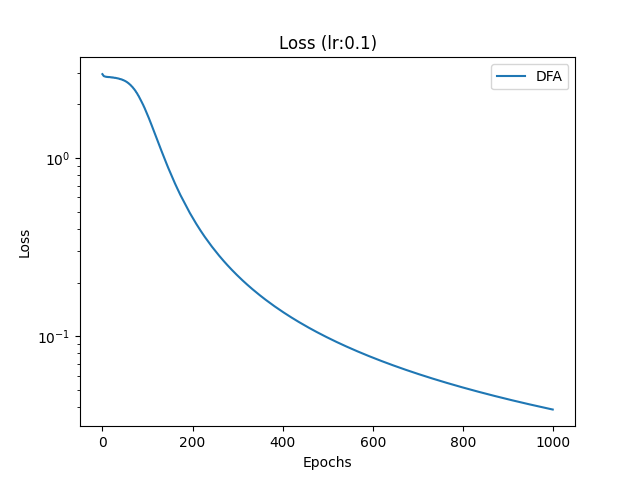
\includegraphics[width=\linewidth]{rsc/XOR/XOR_proofofconcept_LOSS.png}
        \caption{Loss Plot for XOR Proof of Concept}\label{fig:XOR_loss}
    \end{minipage}%
    \hfill
    \begin{minipage}{0.48\textwidth}
        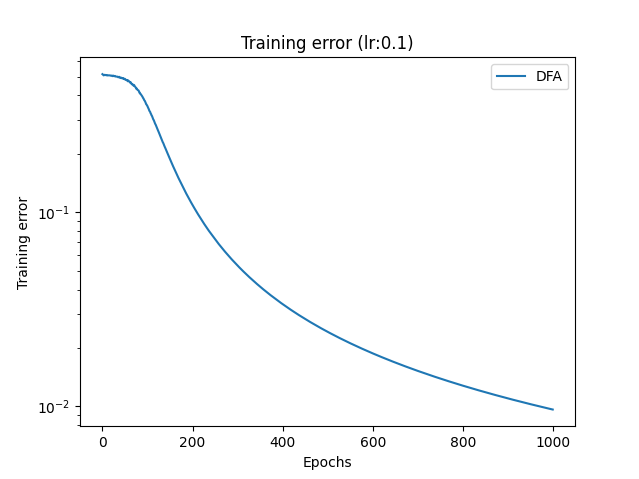
\includegraphics[width=\linewidth]{rsc/XOR/XOR_proofofconcept_TE.png}
        \caption{Training Error Plot for XOR Proof of Concept}\label{fig:XOR_te}
    \end{minipage}%
\end{figure}







\subsection{DFA vs Backpropagation}

% DFA = Direct feedback alignment
% - now using MNIST for a harder problem since the proof of concept works
% - comparing DFA and backpropagation
% - using for training : 500 per batch, 1e-1 learning rate, 200 epochs, architecture is 28*28=784 input, 80 hidden, 10 output (10 digits)
% - include rsc/DFA_BACK/DFA_Back_COMP_LOSS.png and rsc/DFA_BACK/DFA_Back_COMP_TE.png and explain in a paragraph that since DFA only uses the error y_hat - y instead of the loss, comparing the loss does not mean much as it can be shown in the plot. Their values are completely different, whereas the training error matches.

% -we spot that DFA converges down faster than Backprop but that Backprop catches up and converges faster in the long run. However this is not always the case. We suppose that this is due to 

% - we have accuracies of around 97% for training on 200 epochs

% -include rsc/DFA_BACK/DFA_Back_COMP_TE_DFA_close.png, rsc/DFA_BACK/DFA_Back_COMP_TE_DFA_leading.png, rsc/DFA_BACK/DFA_Back_opti_mat_to_std=1.8.png. In a paragraph explain that different situations have been observed, where in DFA_close, backprop and dfa end up on the same line, and where DFA_leading has the DFA leading ahead of backprop. 
% - Make another paragraph that explains that we use a normal distribution to initialize the random B matrices. we used the standard `randn` function of pytorch which has for default parameters mean=0, std=1. However, when using std=1.8, we obtained performance that were better than the backprop Playing with the mean only resulted with worse performance each time. As such we suppose that it would be a good idea to play around with matrices initialization to optimize the convergence rate, first with the std of a normal distribution, but using an alternative distribution may reveal some better results.
% -state that we however kept using a std=1 for the rest of this project, as the std trick was discovered at the end of the allocated time.



Direct Feedback Alignment (DFA) is now being used for a more challenging problem with MNIST, since the proof of concept has already been validated. We compare DFA with traditional backpropagation using a training setup with 500 samples per batch, a learning rate of \(1 \times 10^{-1}\), and 200 epochs. The architecture consists of an input layer of size 784 (from the 28x28 images), an 80-node hidden layer, and an output layer with 10 nodes for the 10 digits.

Fig.\ref{fig:DFA_BACK_te} depicts the training error (TE) over epochs for both methods, highlighting their similar performance in terms of reducing the error. This plot demonstrates that both Direct Feedback Alignment (DFA) and backpropagation effectively minimize the training error during the learning process.


\begin{figure}[!h]
    \centering
    \begin{minipage}{0.48\textwidth}
        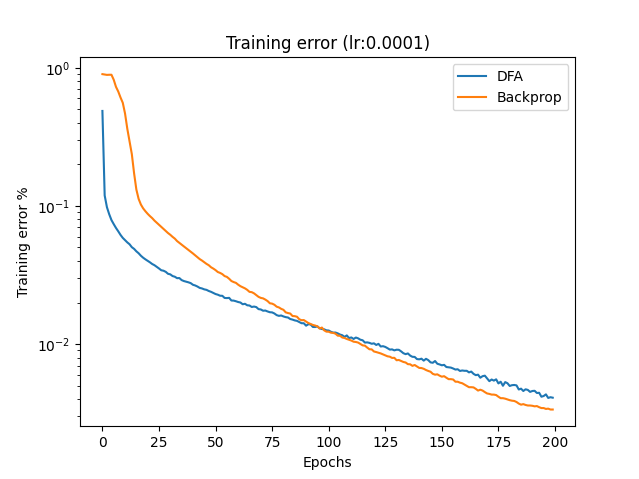
\includegraphics[width=\linewidth]{rsc/DFA_BACK/DFA_Back_COMP_TE.png}
        \caption{Training error (TE) over epochs for both methods}\label{fig:DFA_BACK_te}
    \end{minipage}%
    \hfill
    \begin{minipage}{0.48\textwidth}
        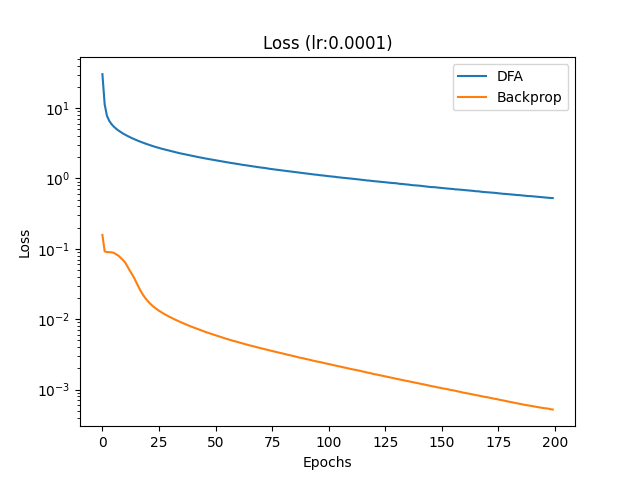
\includegraphics[width=\linewidth]{rsc/DFA_BACK/DFA_Back_COMP_LOSS.png}
        \caption{Comparison of losses between DFA and backpropagation.}\label{fig:DFA_BACK_loss}
    \end{minipage}%
\end{figure}




Fig.\ref{fig:DFA_BACK_loss} illustrate that comparing losses directly can be misleading due to the differing scales of DFA and backpropagation. Here, BP uses RMSELoss while DFA is defined with an error computed using \(e = \hat y - y \). As such, for the DFA we accumulate the error instead of computing the RMSELoss. However, their training errors align quite closely. Specifically, both methods exhibit similar performances in terms of reducing the error over epochs.



\begin{figure}[H]
    \centering
    \begin{minipage}{0.48\textwidth}
        \centering
        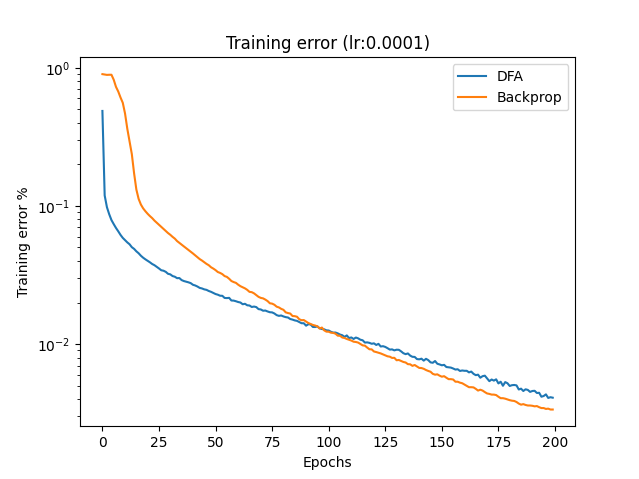
\includegraphics[width=\linewidth]{rsc/DFA_BACK/DFA_Back_COMP_TE.png}
    \end{minipage}%
    \begin{minipage}{0.48\textwidth}
        \centering
        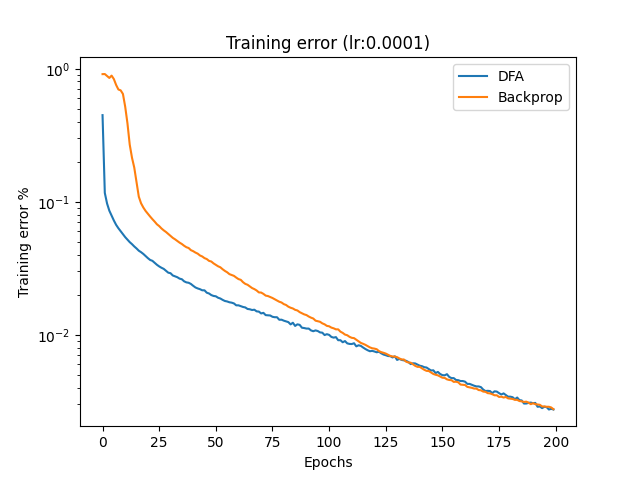
\includegraphics[width=\linewidth]{rsc/DFA_BACK/DFA_Back_COMP_TE_DFA_close.png}
    \end{minipage}%
    \\
    \begin{minipage}{0.48\textwidth}
        \centering
        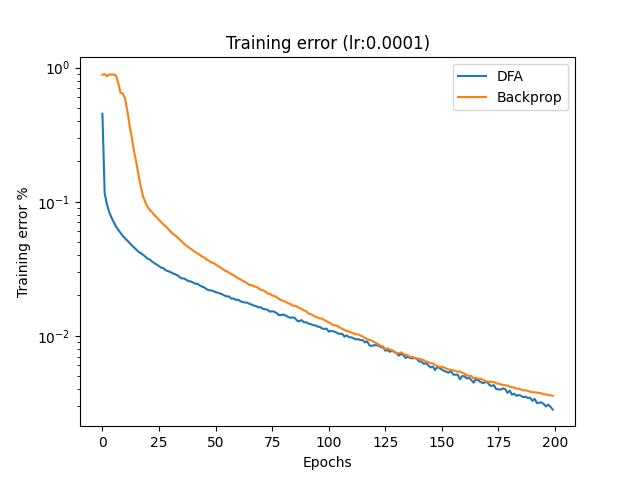
\includegraphics[width=\linewidth]{rsc/DFA_BACK/DFA_Back_COMP_TE_DFA_leading.png}
    \end{minipage}%
    \caption{Comparison of training error (TE) and performance between Direct Feedback Alignment (DFA) and backpropagation.}
\label{fig:DFA_BACK_group}
\end{figure}








% In some cases, as illustrated in the following figures:
% \begin{itemize}
%     \item Fig.\ref{fig:close_convergence} shows a scenario where both methods converge to similar performance levels.
%     \item Fig.\ref{fig:leading_performance} demonstrates instances where DFA leads and performs better than backpropagation.
% \end{itemize}



We also found that initial matrix \( B \) values are crucial for the performance of both methods. We usually initialized these matrices using a normal distribution with mean 0 and standard deviation (std) set to \(\sigma=1\), as provided by PyTorch's `randn()` function. However after fiddling with the matrices initialization, we've found out that different initialization leads to different convergence, explaining the different behaviors in Fig.\ref{fig:DFA_BACK_group}.

After a quick analysis and tests, we settled at \(\sigma=1.9\). Interestingly, this initialization led to better performance compared to backpropagation. Playing with only the mean parameter resulted in consistently worse performance. Thus, we hypothesize that optimizing the initial matrix standards deviations can significantly improve convergence rates.

Please note that this behavior was discovered close to the end of the allocated time for this project. As such, this behavior was not extensively researched.  We can however infer some early hypothesis from our current results

\begin{figure}[h!]
    \centering
    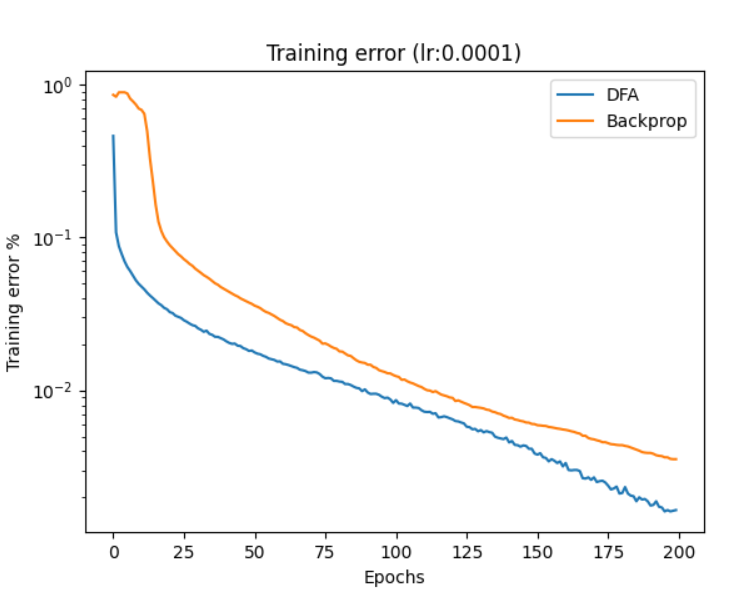
\includegraphics[width=0.48\textwidth]{rsc/DFA_BACK/DFA_Back_opti_mat_to_std=1.8.png}
    \caption{Comparison of training error between optimized DFA and unoptimized backpropagation, with \(B\) matrices initialized using a normal distribution of \(\sigma=1.9\)}\label{fig:DFA_BACK_group}
\end{figure}

As we can see on Fig.\ref{fig:DFA_BACK_group}, the DFA outperforms backpropagation. This is however impossible. It is mathematically certain that DFA cannot outperform Backpropagation\cite{2016arXiv160901596N}. The current behavior is an artefifact of the fact that while we optimized hyper parameters for the DFA, the backpropagation is unoptimized. 

However, for the remainder of our project, we continued using a standard deviation of 1, as the optimal \(\sigma\) was discovered late in the allocated time.

In summary, these observations highlight the importance of careful initialization and suggest that further exploration into alternative distributions might yield even better results.

















\subsection{Gradient angles between DFA and backpropagation}
% - here we compute for each batch we clone the model.
% - we update one of the model using DFA and the second one using backpropagation. 
% - we then compute the angles of the gradiens for each layer between the DFA and backpropagation models
% - finally we plot the result.
% - include here images rsc/angles/DFA_BACK_angles_TE.png and rsc/angles/DFA_BACK_angles.png
% - explain that if angles converge then that means that DFA and backprop tends towards the same optimized ANN.
% - here they do not converge and the angle seems to oscillate around a stable value. as such it seems that DFA and backpropagation do not seem to tend toward the same optimized network. 


Here we compute the angles between the gradients of a neural network optimized using DFA and one optimized using traditional backpropagation for each batch in our training process. Specifically, for each batch, we first clone the models to ensure independent optimization paths. One model is updated using DFA while the other uses backpropagation. We then compute the angles between the gradients of these two models for each layer. The angle is accumulated through one full epoch before being appended to a list and reset. 

The angles are computed using the following mathematical equation:
\[
\theta = \arccos\left(\frac{\mathbf{v}_1 \cdot \mathbf{v}_2}{\|\mathbf{v}_1\| \|\mathbf{v}_2\|}\right)
\]
where \(\mathbf{v}_1\) and \(\mathbf{v}_2\) are the flattened vectors of gradients from the DFA-optimized model and the backpropagation-optimized model, respectively. The dot product \(\mathbf{v}_1 \cdot \mathbf{v}_2\) is computed for each layer, followed by normalizing these vectors to find their magnitudes \(\|\mathbf{v}_1\|\) and \(\|\mathbf{v}_2\|\). This process is repeated for every parameter in the respective layers.

Finally, we plot the results of these angle computations. Fig.\ref{fig:angles-dfa-back} shows the computed angles for each layer across different training epochs. As can be observed, the angles do not converge but rather oscillate around a stable value. This suggests that DFA and backpropagation do not tend toward the same optimized network structure.

To further illustrate this, Fig.\ref{fig:angles-dfa-back-te} presents the training error. A peculiar result is that backpropagation seems to always provide a better update step, being under DFA. However, as we've seen in a previous section, DFA leads. It appears that DFA and Backpropagation minimize the loss function using different directions in the parameter space.



\begin{figure}[!h]
    \centering
    \begin{minipage}{0.48\textwidth}
        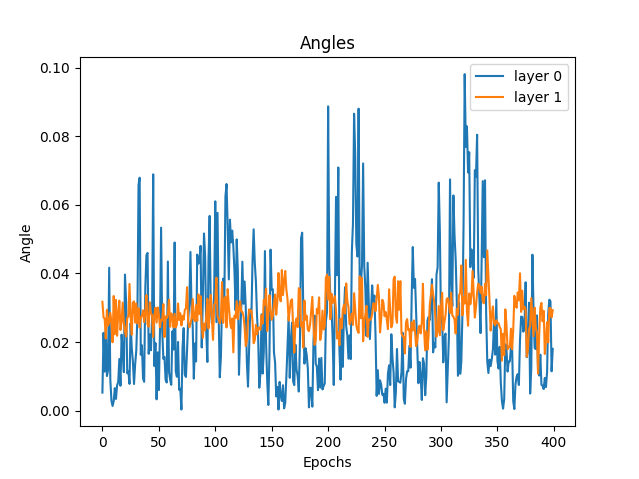
\includegraphics[width=\textwidth]{rsc/angles/DFA_BACK_angles.png}
        \caption{Angles between gradients of DFA and backpropagation-optimized models across different training batches.}\label{fig:angles-dfa-back}
    \end{minipage}%
    \hfill
    \begin{minipage}{0.48\textwidth}
        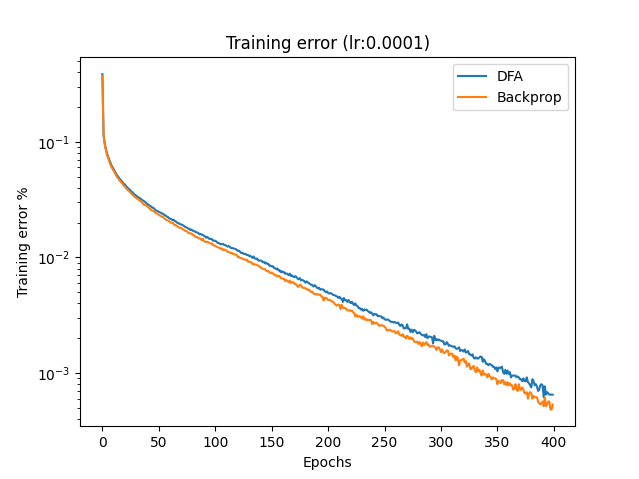
\includegraphics[width=\textwidth]{rsc/angles/DFA_BACK_angles_TE.png}
        \caption{Training error resulting from a backpropagation and DFA optimization step.}\label{fig:angles-dfa-back-te}
    \end{minipage}%
\end{figure}














\subsection{Averaging on a Batch}
% - here we average all the outputs of the batch in a "master" output.
% - here we average all the inputs of the batch in a "master" input.
% - here we average all the targets of the batch in a "master" target.
% - we do the same with the a and h.
% - we compute the error between the master input and and master target.
% - we update the network only using the error, which reduces the number of updates to 1

% in code the update is done like so :
% ```python
% for batch_x, batch_y in dataloader:
%             # Forward pass
%             a, h, y_hat = model.forward_pass_train(batch_x)

%             # Error and error metric
%             error = y_hat - batch_y # used only for metric, recomputed later using averaged
%             preds = torch.argmax(y_hat, dim=0)
%             truth = torch.argmax(batch_y, dim=0)
%             train_error += (preds != truth).sum().item()

%             # Loss metric
%             loss_on_batch = F.binary_cross_entropy(y_hat, batch_y)
%             epoch_loss += loss_on_batch.item()


%             # ======== averaging stuff ============
%             for i in range(len(a)):
%                 a[i] = torch.mean(a[i], dim=0).unsqueeze(0)

%             for i in range(len(h)):
%                 h[i] = torch.mean(h[i], dim=0).unsqueeze(0)

%             y_hat = torch.mean(y_hat, dim=0).unsqueeze(0)
%             batch_y = torch.mean(batch_y, dim=0).unsqueeze(0)
%             batch_x = torch.mean(batch_x, dim=0).unsqueeze(0)
%             # ====================================

%             # Recompute error using averaged batches
%             error = y_hat - batch_y


% ```
% From the code extract the latex formula of how averages are performed for y_hat and batch_y, batch_x, a and h

% - It appears to work at the start for batch sizes where the number of batch is small compared to the number of labels. This is because batches are skewed towards one label. However if we raise the batch size it falls appart because the distribution of labels in batches tends towards a normal distribution.
% - network cannot learn from normal distribution averages because averaging on the batch tends towards the distinctive features of what a digit is, and not towards features of specific digits.
% - explain the point above by noting that using an example where we feed 10 cat images and 10 dog images, then the network cannot know the difference between a dog and a cat because the average label is 50/50 between cats and dogs, but that if we do 1 cats and 9 dogs, it can because the average label is 9/1 dog.



Here we describe a method where, for each batch, all outputs are averaged into a "master" output, and similarly, all inputs and targets are also averaged. The same process is applied to the intermediate variables \(a\) and \(h\). This approach involves computing an error between the master input and the master target, which then updates the network in one step.

The averaging of \(\hat y\) (the model's output) and \(\text{batch\_y}\) (the actual targets) is performed using the following equation:
\begin{equation*}
\text{master\_output} = \frac{1}{N} \sum_{i=1}^{N} \hat y_{i}, \quad \text{master\_target} = \frac{1}{N} \sum_{i=1}^{N} y_{i}
\end{equation*}

where \(N\) is the batch size. Similarly, for inputs and intermediate variables:
\begin{equation*}
        \text{master\_input} = \frac{1}{N} \sum_{i=1}^{N} x_i, \quad \text{master\_h}  = \frac{1}{N} \sum_{i=1}^{N} h_i, \quad \text{master\_a}     = \frac{1}{N} \sum_{i=1}^{N} a_i
\end{equation*}

These equations are applied in the context of training, where \(x\) represents the input data, and \(\hat y\) represents the predicted outputs. The error is then computed as:
\[
\text{error} = \text{master\_output} - \text{master\_target}
\]

This method significantly reduces the number of updates to one per batch, but it faces challenges when dealing with uniform label distributions within batches.

It appears that this approach works well for small batch sizes where labels are not evenly distributed. For instance, consider a scenario where we have 10 cat images and 10 dog images. In such cases, the average target label will be 50/50 between cats and dogs, making it difficult for the network to learn the distinct features of each class. However, if we use batches with only 1 cat image and 9 dog images, the average label would skew towards representing a dog, thereby facilitating better learning.

On increasing the batch size, the distribution of labels tends towards a normal distribution, leading to an averaged output that is less distinctive. For example, averaging 100 images where each class is equally represented (50 cats and 50 dogs) results in an average label that does not favor either category strongly, making it challenging for the network to learn specific features. 

This phenomenon can be illustrated with a simple numerical example: suppose we have two categories, A and B, and our batch consists of images from these categories. If the labels are averaged over a small number of samples (e.g., 10), the resulting average might be heavily skewed towards category A if there are more instances of A in the batch. Conversely, with larger batches where the distribution is closer to equal, averaging would result in an almost neutral output.

\begin{figure}[ht]
    \centering
    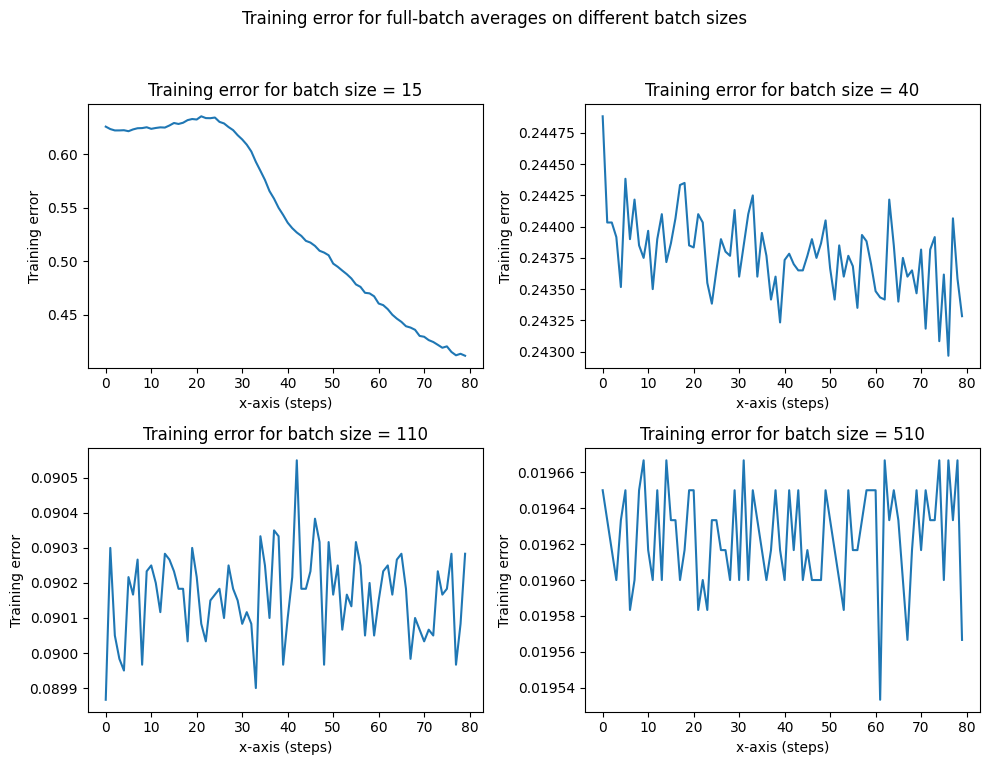
\includegraphics[width=0.8\textwidth]{rsc/full-batch-avg/2x2_TE_grid.png}
    \caption{Effect of Batch Size on the training error when using MNIST dataset (10 labels).}
    \label{fig:batch_size_effect}
\end{figure}

In Figure~\ref{fig:batch_size_effect}, it clearly appears that when the batch is biased towards a specific label due to  undersampling, it will still learn features. However as the batch size increases, the average label tends towards a neutral state, reducing the network's ability to learn distinctive features. This is clearly shown by the graphs. While a size of 40 still leads to a decreasing tendency, 110 and 510 are simply too high to show any sign of convergence. However, 15 shows a typical convergence, albeit quite slow.

While this method ensures that the network is trained using a representative average of the batch, it can lead to suboptimal learning when labels are uniformly distributed. Averaging on a batch helps reduce the number of updates but will lead to suboptimal convergence rates and performance. Smaller batch sizes with skewed distributions facilitate better learning of distinctive features, while larger batches tend towards neutral averages, hindering the network's ability to capture these features effectively.    

As such, when using this method, it is important to consider the distribution of labels inside a specific training set. Having control on the skewing is critical for performance.









\subsection{Averaging per class on a batch }

% - here we separrate the batch per class instead of the whole batch.
% - here we average all the inputs of the batch per class in N_class "master" input. where N_class is the number of class
% - here we average all the targets of the batch per class in N_class "master" target. where N_class is the number of class
% - we do the same with the a and h.
% - we compute the term by term error between the N_i master input and and N_i master target. where N_i is the idex of the class 
% - we update the network only using the N_i errors, which reduces the number of updates to N_i


% ```python
% for batch_x, batch_y in dataloader:
% # Forward pass
% a, h, y_hat = model.forward_pass_train(batch_x)

% # Error and error metric
% error = y_hat - batch_y # used only for metric, recomputed later using averaged
% preds = torch.argmax(y_hat, dim=0)
% truth = torch.argmax(batch_y, dim=0)
% train_error += (preds != truth).sum().item()

% # Loss metric
% # loss_on_batch = nn.CrossEntropyLoss()(y_hat, batch_y)
% loss_on_batch = F.binary_cross_entropy(y_hat, batch_y)
% epoch_loss += loss_on_batch.item()


% # print(batch_y)
% # print(y_hat)
% # print(a)

% # ======== averaging stuff ============

% # get batch indices relevant to the classes
% class_indices = [ [] for _ in range(classes)]
% for item in range(len(batch_y)):
%     class_indices[np.argmax(batch_y[item])].append(item)

% # print(indices)
% # quit()

% # loop over all classes
% for indices in class_indices:

%     if indices == []:
%         continue
%     # print(indices)


%     # ======== averaging over a subset ==========
%     subset_a = []
%     subset_h = []
    
%     # Assuming indices is a list or tensor of indices to average over
%     for i in range(len(a)):
%         subset_a.append(torch.mean(a[i][indices], dim=0).unsqueeze(0))

%     for i in range(len(h)):
%         subset_h.append(torch.mean(h[i][indices], dim=0).unsqueeze(0))

%     sub_y_hat = torch.mean(y_hat[indices], dim=0).unsqueeze(0)
%     sub_batch_y = torch.mean(batch_y[indices], dim=0).unsqueeze(0)
%     # batch_x = torch.mean(batch_x[indices], dim=0).unsqueeze(0)
%     # ==========================================

%     # Recompute error using averaged batches
%     error = sub_y_hat - sub_batch_y

%     # print('subset_a\n',subset_a)
%     # Transposition of a and h for dimensions match
%     sub_a = [matrix.T for matrix in subset_a]
%     sub_h = [matrix.T for matrix in subset_h]


%     # DFA backward pass
%     dW, db = model.dfa_backward_pass(error.T, sub_h, sub_a, B)

%     # Update weights manually
%     with torch.no_grad():
%         for i in range(len(db)):
%             model.layers[i].weight += lr * dW[i]
%             model.layers[i].bias += lr * db[i].squeeze()
% ```
% From the code extract the latex formula of how averages are performed for y_hat and batch_y, batch_x, a and h

% - include image rsc/class-batch-avg/lr_sweep.png where we sweep the learning rate on a batch size of 500.
% - The above image shows that learning rate is critical. if too high it will not do anything and not learn because the steps are too big to converge in local minimas. if too small the convergence will take way too long. we spot a plateau at the start which seems to correspond to a pre-alignment of the network, before converging to a local minima. we denote that this plateau and the convergence rate is dependent on the learning rate. As such we submit the hypothesis that using a learning rate schedule to shorten the time spent plateauing is a good idea. We also suggest to optimize the B matrices initialization as seen in section 4.3. 


% - include image rsc/class-batch-avg/batch_sweep.png where we sweep the batch size with a learning rate of 0.001.
% - the above image shows that the batch size impacts the convergence speed/epoch. This is due to the fact that the network receives less updates per epochs with bigger batch sizes. However, bigger batch size still leads to convergence. This is a very good result for experimentalists where it is possible to extract separate labels during integration time on the system. it is important to note that numerically speaking, while bigger batch coverges slowly, the computation time necessary for smaller batch size is way superior; as such we would recommend to include the time per epoch in the comparison.



In this section, we describe the process of averaging inputs, targets, and intermediate representations per class within a batch during training. This approach helps reduce the number of updates to the network while retaining meaningful gradient information for each class.

We begin by separating the batch into subsets corresponding to each class. For a batch containing $N$ samples and $C$ classes, we group indices of the samples based on their class label. Denoting $\mathbf{y}_\text{batch}$ as the target labels and $\mathbf{\hat{y}}_\text{batch}$ as the model predictions, the averaging operations for each class $i$ are expressed as:
\[
\mathbf{\hat{y}}_i = \frac{1}{|S_i|} \sum_{j \in S_i} \mathbf{\hat{y}}_j, \quad
\mathbf{y}_i = \frac{1}{|S_i|} \sum_{j \in S_i} \mathbf{y}_j,
\]
where $S_i$ is the set of indices for samples belonging to class $i$, and $|S_i|$ is the size of this set. Similar averaging is performed for the intermediate activations $\mathbf{a}$ and $\mathbf{h}$:
\[
\mathbf{a}_i = \frac{1}{|S_i|} \sum_{j \in S_i} \mathbf{a}_j, \quad
\mathbf{h}_i = \frac{1}{|S_i|} \sum_{j \in S_i} \mathbf{h}_j.
\]
This process reduces the computational overhead by averaging over the class-specific subsets instead of updating the network for each individual sample.

\subsubsection{Impact of Learning Rate}

Figure~\ref{fig:lr_sweep} illustrates the impact of varying the learning rate on convergence behavior for a batch size of 500. The results show that the choice of learning rate is critical. A high learning rate prevents the model from converging due to large update steps that fail to settle in local minima. Conversely, a very small learning rate significantly increases convergence time. We observe a plateau at the beginning of training, which likely corresponds to an initial pre-alignment of the network before converging to a local minimum. Notably, the duration of this plateau and the overall convergence rate are dependent on the learning rate.

Based on these observations, we hypothesize that employing a learning rate schedule could shorten the time spent in the plateau phase, thereby accelerating convergence. Additionally, optimizing the initialization of the feedback matrices $\mathbf{B}$, as discussed in Section~4.3, may further improve convergence performance.

\begin{figure}[H]
    \centering
    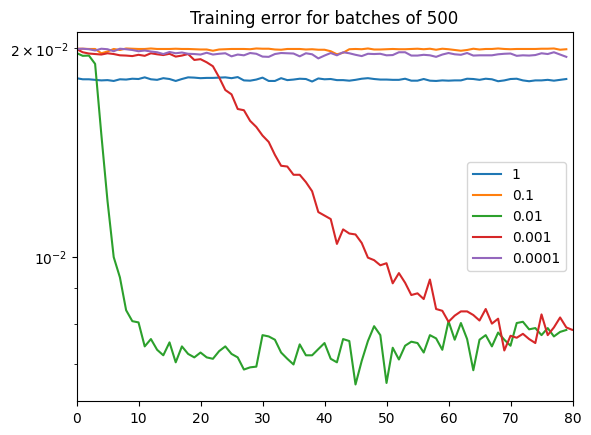
\includegraphics[width=0.48\textwidth]{rsc/class-batch-avg/lr_sweep.png}
    \caption{Impact of learning rate on convergence for a batch size of 500.}
    \label{fig:lr_sweep}
\end{figure}

\subsubsection{Impact of Batch Size}

Figure~\ref{fig:batch_sweep} shows the effect of batch size on convergence speed per epoch, using a fixed learning rate of 0.001. Larger batch sizes result in fewer updates per epoch, slowing convergence speed in terms of epochs. However, convergence is still achieved even with larger batch sizes. This is particularly promising for experimental setups where extracting separate labels during integration time is feasible.

It is worth noting that while smaller batch sizes converge faster in terms of epochs, the computational time required for each epoch is significantly higher. For practical applications, it is essential to also account for time per epoch when comparing the efficiency of different batch sizes.

\begin{figure}[H]
    \centering
    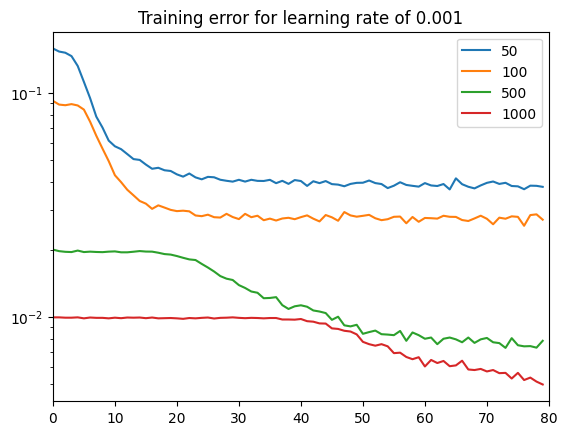
\includegraphics[width=0.48\textwidth]{rsc/class-batch-avg/batch_sweep.png}
    \caption{Impact of batch size on convergence with a fixed learning rate of 0.001.}
    \label{fig:batch_sweep}
\end{figure}








\section{Conclusion}
In this project, we explored the implementation and application of Direct Feedback Alignment (DFA) as an alternative to backpropagation for training neural networks. Our results demonstrate that DFA successfully minimizes training loss and error in both simple and complex problems, such as the XOR and MNIST datasets, validating its potential as a training method.

Key findings include the sensitivity of DFA's performance to the initialization of weight matrices and the significance of hyperparameter optimization. While DFA performed comparably to backpropagation in terms of error reduction, further investigation revealed that its performance could be enhanced by fine-tuning initialization parameters, such as the standard deviation of matrix \(B\). However, it was also observed that this improvement did not inherently indicate superiority over backpropagation but rather reflected the lack of equivalent optimization for both methods during the experiments.

Additional experiments on gradient angles confirmed that DFA and backpropagation utilize different optimization trajectories, emphasizing the distinct mechanisms underlying these methods. Moreover, the averaging strategies explored in the batch and class-specific contexts provided insights into the trade-offs between computational efficiency and model convergence. Smaller batch sizes with skewed distributions proved beneficial for feature learning, while larger batches hindered convergence due to neutral averaging effects.

While DFA offers a promising alternative to backpropagation, its limitations, such as sensitivity to initialization and hyperparameter selection, warrant further research. Future work could focus on improving DFA's robustness and exploring its applicability to diverse architectures and datasets. Overall, this study highlights the potential of DFA and lays the groundwork for advancing understanding and application of alternative training methods in neural networks, especially in regads to averaged batches in training.

















% \begin{figure}[H]
%   \begin{center}
%     \includegraphics[scale=0.5]{8_oct_ref_star and sat.png}
%     \caption{Position of the Asteroid and Star During the First Observation on October 8th}
%     \label{origine 8}
%   \end{center}
% \end{figure}


% \begin{equation}
%         C_F^* = r - mag_i^{cal*}
%         \label{CF}
% \end{equation}\\







% \newpage
% \begin{appendix}
% \section{Appendix}



% \end{appendix}


\bibliography{references} 
\bibliographystyle{ieeetr}

\end{document}